%%% ================= Preamble =========================
\documentclass[12pt]{umthesis}
\usepackage{amsmath}
\usepackage{amsfonts}
\usepackage{cleveref}
\usepackage{apacite}
\usepackage{graphicx}
\usepackage{adjustbox}
\usepackage[font=small,labelfont=bf]{caption}
\usepackage{url}
\usepackage{lineno}
\usepackage{soul}
\usepackage{fix-cm}
\usepackage{textcomp}
\usepackage{multirow}
\usepackage{longtable}
\usepackage{booktabs}
\usepackage{tabularray}
\usepackage{chngcntr}
\usepackage{CJKutf8}

%%% =============== Title, author, committe members=====
\thesistitle{AN UNOFFICIAL THESIS TEMPLATE FOR UMASS AMHERST GRADUATE STUDENTS}
\thesisauthor{Xinchen He}
\thesisdept{Civil and Environmental Engineering}
\thesisdate{May 2025}
\prevdegree{B.S., XXX University; M.S., YYY University} % previous academic degrees
% Name of your committe member
\committeechair{FirstName LastName} % committe chair
\firstreader{FirstName LastName} % committe member 1
\secondreader{FirstName LastName}% committe member 2
\outsidereader{FirstName LastName}% committe member 3, outside your department
\depthead{Sergio Brena} % department head

\advisorname{Professor FirstName LastName; Professor FirstName LastName} % name of your advisor(s) with their titles. This would appear in the heading of the abstract

% Acknowledgement
\thesisacknowledgment{I would like to thank...}

% Abstract
\thesisabstract{Abstract of your thesis}


% Document begin
\begin{document}

% Preface
\pagenumbering{roman}
\maketitlepage
\makecopyrightpage
\makesignaturepage
\makeacknowledgmentpage
\makeabstractpage
% Table of content
\tableofcontents
\pagebreak
\addcontentsline{toc}{part}{LIST OF TABLES}
\listoftables
\pagebreak
\addcontentsline{toc}{part}{LIST OF FIGURES}
% Add vertical space before CHAPTER
\addtocontents{toc}{\protect\vspace{2pt}}
\addtocontents{toc}{\bfseries CHAPTER \par}
\listoffigures
\pagebreak
\newpage
\cleardoublepage
\pagenumbering{arabic}
\setcounter{page}{1}

% Chapters
\chapter{INTRODUCTION}

\section{Overall structure}

- thesis.tex: The main LaTeX document. Compile this file to generate the PDF of your dissertation.

- references.bib: The bibliography file that stores the BibTeX entries of your referenced literature.

- chapters/: A directory containing individual .tex files for each of your thesis chapters. Please replace the placeholder content with your own chapters. Ensure that all figures are correctly referenced.

- figs/: A directory for storing your figure files. It is recommended to organize figures by chapter.

- appendix/: This folder contains supplementary materials, organized by chapter.

\section{Citation}

For citations, please use \verb|\cite{}| or \verb|\citeA{}| to reference literature included in your BibTeX file (e.g., references.bib). For example, global warming has led to widespread lake ice loss over the past century \cite{Huang2022Oct, Sharma2019Mar}. \citeA{He2025Jun} used an LSTM model to simulate daily lake ice cover in the Northern Hemisphere.

\section{Cross reference}

For cross-referencing figures and tables, this template uses the cleveref package, which allows you to reference figures, tables, and sections using \verb|\cref{label}|. For example, \cref{iceloss} shows changes in lake ice intermittency over the past four decades in the Northern Hemisphere; \cref{inputtable} lists the input and output variable of the lake ice model.

\begin{figure}[ht]
\centering
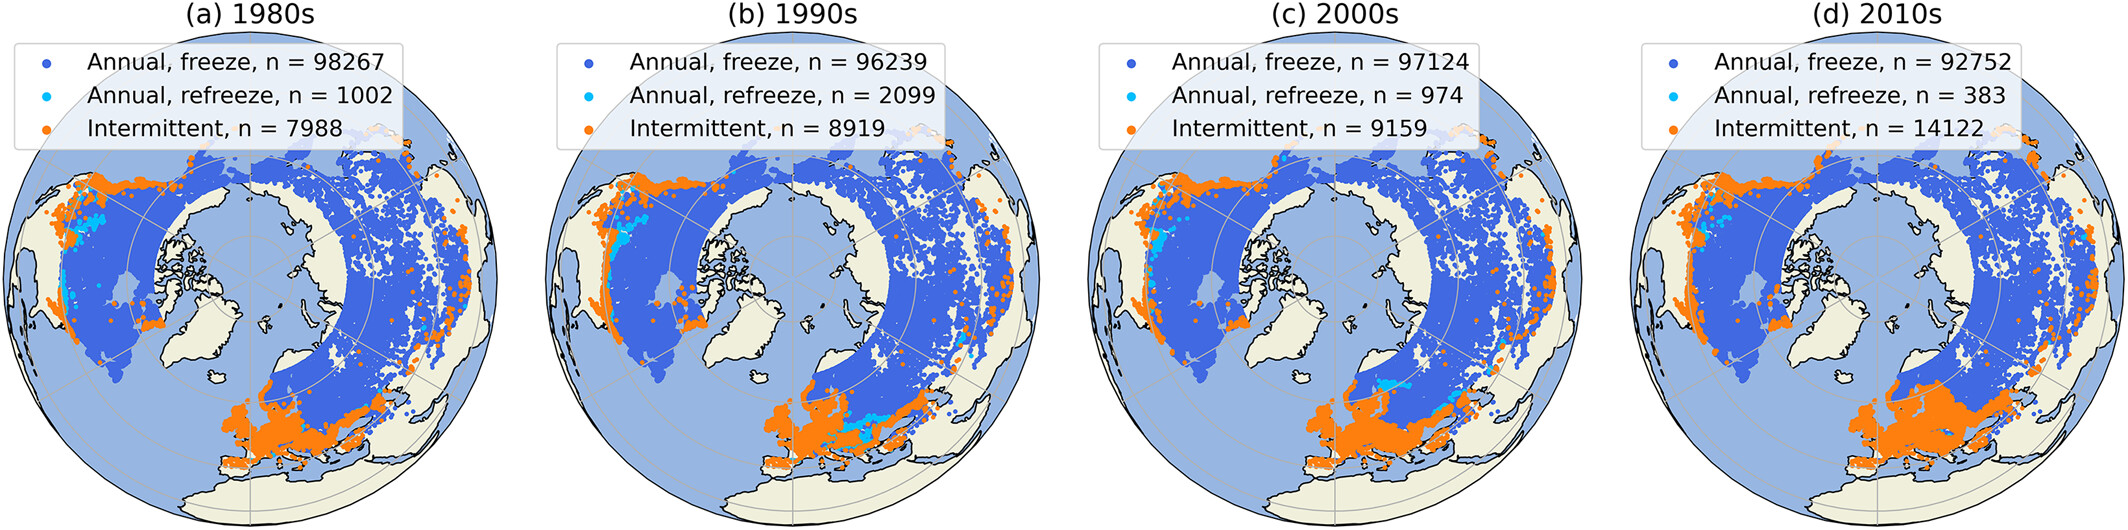
\includegraphics[width=\textwidth]{figs/ch1/iceloss.jpg}
\caption{Geographic distribution of lake ice intermittency over the past four decades. "Annual, refreeze" represents the annually ice-covered lakes which experienced multiple freeze-thaw events during the decade, while the "Annual, freeze" lakes did not experience multiple freeze-thaw events.}
\label{iceloss}
\end{figure}

\begin{table}[ht]
\caption{Summary of the input and output variables for the Long Short Term Memory (LSTM) lake ice cover model. $K$ = Kelvin, $J$ = Joule, $mcm$ = million cubic meters},
\resizebox{\linewidth}{!}{
\begin{tabular}{cccc}
\hline
Group & Variable Name & Description & Unit \\
\hline
Output & Ice Cover & The ratio of ice covered area and total lake surface area & \textbackslash{} \\
Input: Forcings & t2max & daily maximum air temperature at 2 meters above the earth surface & $K$ \\
 & t2min & Daily minimum air temperature at 2 meters above the earth surface & $K$ \\
 & srad & Daily averaged solar radiation downward to the earth surface & $J/m^2$ \\
 & u10 & Eastward windspeed at 10 meters above the earth surface & $m/s$ \\
 & v10 & Northward windspeed at 10 meters above the earth surface & $m/s$ \\
 & tp & Total precipitation & $m$ \\
Input: Lake attributes & Lake\textunderscore area & Lake surface area & $km$ \\
 & Vol\textunderscore total & Total lake or reservoir volume & $mcm$ \\
 & Shore\textunderscore len & Shoreline length & $km$ \\
 & Res\textunderscore time & Average residence time of the lake water & $days$ \\
 & Elevation & Elevation of lake surface & $m$\\
\hline
\end{tabular}
}
\label{inputtable}
\end{table} % usually the first chapter is a general introduction
\chapter{CHAPTER 2}
\section{Abstract}
Lorem ipsum dolor sit amet, consectetur adipiscing elit. Ut mi ante, mollis auctor turpis et, mollis rhoncus lacus. Aliquam euismod volutpat nisi nec commodo. Donec eu leo id leo consequat dictum eget sed elit. Morbi et tempor nunc. Ut et nibh nec justo scelerisque cursus. Proin mollis, erat eu elementum lobortis, enim eros cursus odio, viverra porta odio mi sed purus. Nulla ut eleifend nisl. Donec laoreet eros sed elit finibus blandit. Nunc quis varius ex. Proin lectus mauris, aliquam et justo nec, tincidunt mattis risus. Aenean est est, elementum vel quam non, facilisis blandit est.

Aenean vel nisl vel leo scelerisque scelerisque nec nec lorem. Sed ac sem eget ante porttitor egestas. Donec quis gravida ex, et bibendum nulla. Mauris condimentum urna leo, eu bibendum lorem vulputate quis. Vivamus ullamcorper tincidunt ex, sed sagittis dolor interdum sed. Proin auctor, est ac dictum ullamcorper, justo magna porta enim, id varius dolor lorem a ex. Integer accumsan iaculis convallis. Maecenas feugiat volutpat neque, eu egestas enim convallis in. Donec sed purus ut mauris placerat molestie nec vitae tortor.

Suspendisse semper, mi non tempor fermentum, felis tortor tristique dolor, a fringilla sem odio non quam. Donec lacinia tristique pretium. Aliquam nisl mauris, consequat vitae mattis quis, sagittis eget massa. Pellentesque in nisi lobortis, gravida lacus ut, egestas ligula. Ut porta dignissim libero, a sagittis ligula rhoncus eget. Aenean efficitur odio sed lacus pharetra lacinia id eget urna. Aliquam erat volutpat.

\section{Introduction}
Lorem ipsum dolor sit amet, consectetur adipiscing elit. Ut mi ante, mollis auctor turpis et, mollis rhoncus lacus. Aliquam euismod volutpat nisi nec commodo. Donec eu leo id leo consequat dictum eget sed elit. Morbi et tempor nunc. Ut et nibh nec justo scelerisque cursus. Proin mollis, erat eu elementum lobortis, enim eros cursus odio, viverra porta odio mi sed purus. Nulla ut eleifend nisl. Donec laoreet eros sed elit finibus blandit. Nunc quis varius ex. Proin lectus mauris, aliquam et justo nec, tincidunt mattis risus. Aenean est est, elementum vel quam non, facilisis blandit est.

Aenean vel nisl vel leo scelerisque scelerisque nec nec lorem. Sed ac sem eget ante porttitor egestas. Donec quis gravida ex, et bibendum nulla. Mauris condimentum urna leo, eu bibendum lorem vulputate quis. Vivamus ullamcorper tincidunt ex, sed sagittis dolor interdum sed. Proin auctor, est ac dictum ullamcorper, justo magna porta enim, id varius dolor lorem a ex. Integer accumsan iaculis convallis. Maecenas feugiat volutpat neque, eu egestas enim convallis in. Donec sed purus ut mauris placerat molestie nec vitae tortor.

Suspendisse semper, mi non tempor fermentum, felis tortor tristique dolor, a fringilla sem odio non quam. Donec lacinia tristique pretium. Aliquam nisl mauris, consequat vitae mattis quis, sagittis eget massa. Pellentesque in nisi lobortis, gravida lacus ut, egestas ligula. Ut porta dignissim libero, a sagittis ligula rhoncus eget. Aenean efficitur odio sed lacus pharetra lacinia id eget urna. Aliquam erat volutpat.

\section{Methods}
Lorem ipsum dolor sit amet, consectetur adipiscing elit. Ut mi ante, mollis auctor turpis et, mollis rhoncus lacus. Aliquam euismod volutpat nisi nec commodo. Donec eu leo id leo consequat dictum eget sed elit. Morbi et tempor nunc. Ut et nibh nec justo scelerisque cursus. Proin mollis, erat eu elementum lobortis, enim eros cursus odio, viverra porta odio mi sed purus. Nulla ut eleifend nisl. Donec laoreet eros sed elit finibus blandit. Nunc quis varius ex. Proin lectus mauris, aliquam et justo nec, tincidunt mattis risus. Aenean est est, elementum vel quam non, facilisis blandit est.

Aenean vel nisl vel leo scelerisque scelerisque nec nec lorem. Sed ac sem eget ante porttitor egestas. Donec quis gravida ex, et bibendum nulla. Mauris condimentum urna leo, eu bibendum lorem vulputate quis. Vivamus ullamcorper tincidunt ex, sed sagittis dolor interdum sed. Proin auctor, est ac dictum ullamcorper, justo magna porta enim, id varius dolor lorem a ex. Integer accumsan iaculis convallis. Maecenas feugiat volutpat neque, eu egestas enim convallis in. Donec sed purus ut mauris placerat molestie nec vitae tortor.

Suspendisse semper, mi non tempor fermentum, felis tortor tristique dolor, a fringilla sem odio non quam. Donec lacinia tristique pretium. Aliquam nisl mauris, consequat vitae mattis quis, sagittis eget massa. Pellentesque in nisi lobortis, gravida lacus ut, egestas ligula. Ut porta dignissim libero, a sagittis ligula rhoncus eget. Aenean efficitur odio sed lacus pharetra lacinia id eget urna. Aliquam erat volutpat.

\section{Results}
Lorem ipsum dolor sit amet, consectetur adipiscing elit. Ut mi ante, mollis auctor turpis et, mollis rhoncus lacus. Aliquam euismod volutpat nisi nec commodo. Donec eu leo id leo consequat dictum eget sed elit. Morbi et tempor nunc. Ut et nibh nec justo scelerisque cursus. Proin mollis, erat eu elementum lobortis, enim eros cursus odio, viverra porta odio mi sed purus. Nulla ut eleifend nisl. Donec laoreet eros sed elit finibus blandit. Nunc quis varius ex. Proin lectus mauris, aliquam et justo nec, tincidunt mattis risus. Aenean est est, elementum vel quam non, facilisis blandit est.

Aenean vel nisl vel leo scelerisque scelerisque nec nec lorem. Sed ac sem eget ante porttitor egestas. Donec quis gravida ex, et bibendum nulla. Mauris condimentum urna leo, eu bibendum lorem vulputate quis. Vivamus ullamcorper tincidunt ex, sed sagittis dolor interdum sed. Proin auctor, est ac dictum ullamcorper, justo magna porta enim, id varius dolor lorem a ex. Integer accumsan iaculis convallis. Maecenas feugiat volutpat neque, eu egestas enim convallis in. Donec sed purus ut mauris placerat molestie nec vitae tortor.

Suspendisse semper, mi non tempor fermentum, felis tortor tristique dolor, a fringilla sem odio non quam. Donec lacinia tristique pretium. Aliquam nisl mauris, consequat vitae mattis quis, sagittis eget massa. Pellentesque in nisi lobortis, gravida lacus ut, egestas ligula. Ut porta dignissim libero, a sagittis ligula rhoncus eget. Aenean efficitur odio sed lacus pharetra lacinia id eget urna. Aliquam erat volutpat.

\section{Discussion}
Lorem ipsum dolor sit amet, consectetur adipiscing elit. Ut mi ante, mollis auctor turpis et, mollis rhoncus lacus. Aliquam euismod volutpat nisi nec commodo. Donec eu leo id leo consequat dictum eget sed elit. Morbi et tempor nunc. Ut et nibh nec justo scelerisque cursus. Proin mollis, erat eu elementum lobortis, enim eros cursus odio, viverra porta odio mi sed purus. Nulla ut eleifend nisl. Donec laoreet eros sed elit finibus blandit. Nunc quis varius ex. Proin lectus mauris, aliquam et justo nec, tincidunt mattis risus. Aenean est est, elementum vel quam non, facilisis blandit est.

Aenean vel nisl vel leo scelerisque scelerisque nec nec lorem. Sed ac sem eget ante porttitor egestas. Donec quis gravida ex, et bibendum nulla. Mauris condimentum urna leo, eu bibendum lorem vulputate quis. Vivamus ullamcorper tincidunt ex, sed sagittis dolor interdum sed. Proin auctor, est ac dictum ullamcorper, justo magna porta enim, id varius dolor lorem a ex. Integer accumsan iaculis convallis. Maecenas feugiat volutpat neque, eu egestas enim convallis in. Donec sed purus ut mauris placerat molestie nec vitae tortor.

Suspendisse semper, mi non tempor fermentum, felis tortor tristique dolor, a fringilla sem odio non quam. Donec lacinia tristique pretium. Aliquam nisl mauris, consequat vitae mattis quis, sagittis eget massa. Pellentesque in nisi lobortis, gravida lacus ut, egestas ligula. Ut porta dignissim libero, a sagittis ligula rhoncus eget. Aenean efficitur odio sed lacus pharetra lacinia id eget urna. Aliquam erat volutpat.

\section{Conclusion}
Lorem ipsum dolor sit amet, consectetur adipiscing elit. Ut mi ante, mollis auctor turpis et, mollis rhoncus lacus. Aliquam euismod volutpat nisi nec commodo. Donec eu leo id leo consequat dictum eget sed elit. Morbi et tempor nunc. Ut et nibh nec justo scelerisque cursus. Proin mollis, erat eu elementum lobortis, enim eros cursus odio, viverra porta odio mi sed purus. Nulla ut eleifend nisl. Donec laoreet eros sed elit finibus blandit. Nunc quis varius ex. Proin lectus mauris, aliquam et justo nec, tincidunt mattis risus. Aenean est est, elementum vel quam non, facilisis blandit est.

Aenean vel nisl vel leo scelerisque scelerisque nec nec lorem. Sed ac sem eget ante porttitor egestas. Donec quis gravida ex, et bibendum nulla. Mauris condimentum urna leo, eu bibendum lorem vulputate quis. Vivamus ullamcorper tincidunt ex, sed sagittis dolor interdum sed. Proin auctor, est ac dictum ullamcorper, justo magna porta enim, id varius dolor lorem a ex. Integer accumsan iaculis convallis. Maecenas feugiat volutpat neque, eu egestas enim convallis in. Donec sed purus ut mauris placerat molestie nec vitae tortor.

Suspendisse semper, mi non tempor fermentum, felis tortor tristique dolor, a fringilla sem odio non quam. Donec lacinia tristique pretium. Aliquam nisl mauris, consequat vitae mattis quis, sagittis eget massa. Pellentesque in nisi lobortis, gravida lacus ut, egestas ligula. Ut porta dignissim libero, a sagittis ligula rhoncus eget. Aenean efficitur odio sed lacus pharetra lacinia id eget urna. Aliquam erat volutpat.
\chapter{CHAPTER 3}

\section{Abstract}
Lorem ipsum dolor sit amet, consectetur adipiscing elit. Ut mi ante, mollis auctor turpis et, mollis rhoncus lacus. Aliquam euismod volutpat nisi nec commodo. Donec eu leo id leo consequat dictum eget sed elit. Morbi et tempor nunc. Ut et nibh nec justo scelerisque cursus. Proin mollis, erat eu elementum lobortis, enim eros cursus odio, viverra porta odio mi sed purus. Nulla ut eleifend nisl. Donec laoreet eros sed elit finibus blandit. Nunc quis varius ex. Proin lectus mauris, aliquam et justo nec, tincidunt mattis risus. Aenean est est, elementum vel quam non, facilisis blandit est.

Aenean vel nisl vel leo scelerisque scelerisque nec nec lorem. Sed ac sem eget ante porttitor egestas. Donec quis gravida ex, et bibendum nulla. Mauris condimentum urna leo, eu bibendum lorem vulputate quis. Vivamus ullamcorper tincidunt ex, sed sagittis dolor interdum sed. Proin auctor, est ac dictum ullamcorper, justo magna porta enim, id varius dolor lorem a ex. Integer accumsan iaculis convallis. Maecenas feugiat volutpat neque, eu egestas enim convallis in. Donec sed purus ut mauris placerat molestie nec vitae tortor.

Suspendisse semper, mi non tempor fermentum, felis tortor tristique dolor, a fringilla sem odio non quam. Donec lacinia tristique pretium. Aliquam nisl mauris, consequat vitae mattis quis, sagittis eget massa. Pellentesque in nisi lobortis, gravida lacus ut, egestas ligula. Ut porta dignissim libero, a sagittis ligula rhoncus eget. Aenean efficitur odio sed lacus pharetra lacinia id eget urna. Aliquam erat volutpat.

\section{Introduction}
Lorem ipsum dolor sit amet, consectetur adipiscing elit. Ut mi ante, mollis auctor turpis et, mollis rhoncus lacus. Aliquam euismod volutpat nisi nec commodo. Donec eu leo id leo consequat dictum eget sed elit. Morbi et tempor nunc. Ut et nibh nec justo scelerisque cursus. Proin mollis, erat eu elementum lobortis, enim eros cursus odio, viverra porta odio mi sed purus. Nulla ut eleifend nisl. Donec laoreet eros sed elit finibus blandit. Nunc quis varius ex. Proin lectus mauris, aliquam et justo nec, tincidunt mattis risus. Aenean est est, elementum vel quam non, facilisis blandit est.

Aenean vel nisl vel leo scelerisque scelerisque nec nec lorem. Sed ac sem eget ante porttitor egestas. Donec quis gravida ex, et bibendum nulla. Mauris condimentum urna leo, eu bibendum lorem vulputate quis. Vivamus ullamcorper tincidunt ex, sed sagittis dolor interdum sed. Proin auctor, est ac dictum ullamcorper, justo magna porta enim, id varius dolor lorem a ex. Integer accumsan iaculis convallis. Maecenas feugiat volutpat neque, eu egestas enim convallis in. Donec sed purus ut mauris placerat molestie nec vitae tortor.

Suspendisse semper, mi non tempor fermentum, felis tortor tristique dolor, a fringilla sem odio non quam. Donec lacinia tristique pretium. Aliquam nisl mauris, consequat vitae mattis quis, sagittis eget massa. Pellentesque in nisi lobortis, gravida lacus ut, egestas ligula. Ut porta dignissim libero, a sagittis ligula rhoncus eget. Aenean efficitur odio sed lacus pharetra lacinia id eget urna. Aliquam erat volutpat.

\section{Methods}
Lorem ipsum dolor sit amet, consectetur adipiscing elit. Ut mi ante, mollis auctor turpis et, mollis rhoncus lacus. Aliquam euismod volutpat nisi nec commodo. Donec eu leo id leo consequat dictum eget sed elit. Morbi et tempor nunc. Ut et nibh nec justo scelerisque cursus. Proin mollis, erat eu elementum lobortis, enim eros cursus odio, viverra porta odio mi sed purus. Nulla ut eleifend nisl. Donec laoreet eros sed elit finibus blandit. Nunc quis varius ex. Proin lectus mauris, aliquam et justo nec, tincidunt mattis risus. Aenean est est, elementum vel quam non, facilisis blandit est.

Aenean vel nisl vel leo scelerisque scelerisque nec nec lorem. Sed ac sem eget ante porttitor egestas. Donec quis gravida ex, et bibendum nulla. Mauris condimentum urna leo, eu bibendum lorem vulputate quis. Vivamus ullamcorper tincidunt ex, sed sagittis dolor interdum sed. Proin auctor, est ac dictum ullamcorper, justo magna porta enim, id varius dolor lorem a ex. Integer accumsan iaculis convallis. Maecenas feugiat volutpat neque, eu egestas enim convallis in. Donec sed purus ut mauris placerat molestie nec vitae tortor.

Suspendisse semper, mi non tempor fermentum, felis tortor tristique dolor, a fringilla sem odio non quam. Donec lacinia tristique pretium. Aliquam nisl mauris, consequat vitae mattis quis, sagittis eget massa. Pellentesque in nisi lobortis, gravida lacus ut, egestas ligula. Ut porta dignissim libero, a sagittis ligula rhoncus eget. Aenean efficitur odio sed lacus pharetra lacinia id eget urna. Aliquam erat volutpat.

\section{Results}
Lorem ipsum dolor sit amet, consectetur adipiscing elit. Ut mi ante, mollis auctor turpis et, mollis rhoncus lacus. Aliquam euismod volutpat nisi nec commodo. Donec eu leo id leo consequat dictum eget sed elit. Morbi et tempor nunc. Ut et nibh nec justo scelerisque cursus. Proin mollis, erat eu elementum lobortis, enim eros cursus odio, viverra porta odio mi sed purus. Nulla ut eleifend nisl. Donec laoreet eros sed elit finibus blandit. Nunc quis varius ex. Proin lectus mauris, aliquam et justo nec, tincidunt mattis risus. Aenean est est, elementum vel quam non, facilisis blandit est.

Aenean vel nisl vel leo scelerisque scelerisque nec nec lorem. Sed ac sem eget ante porttitor egestas. Donec quis gravida ex, et bibendum nulla. Mauris condimentum urna leo, eu bibendum lorem vulputate quis. Vivamus ullamcorper tincidunt ex, sed sagittis dolor interdum sed. Proin auctor, est ac dictum ullamcorper, justo magna porta enim, id varius dolor lorem a ex. Integer accumsan iaculis convallis. Maecenas feugiat volutpat neque, eu egestas enim convallis in. Donec sed purus ut mauris placerat molestie nec vitae tortor.

Suspendisse semper, mi non tempor fermentum, felis tortor tristique dolor, a fringilla sem odio non quam. Donec lacinia tristique pretium. Aliquam nisl mauris, consequat vitae mattis quis, sagittis eget massa. Pellentesque in nisi lobortis, gravida lacus ut, egestas ligula. Ut porta dignissim libero, a sagittis ligula rhoncus eget. Aenean efficitur odio sed lacus pharetra lacinia id eget urna. Aliquam erat volutpat.

\section{Discussion}
Lorem ipsum dolor sit amet, consectetur adipiscing elit. Ut mi ante, mollis auctor turpis et, mollis rhoncus lacus. Aliquam euismod volutpat nisi nec commodo. Donec eu leo id leo consequat dictum eget sed elit. Morbi et tempor nunc. Ut et nibh nec justo scelerisque cursus. Proin mollis, erat eu elementum lobortis, enim eros cursus odio, viverra porta odio mi sed purus. Nulla ut eleifend nisl. Donec laoreet eros sed elit finibus blandit. Nunc quis varius ex. Proin lectus mauris, aliquam et justo nec, tincidunt mattis risus. Aenean est est, elementum vel quam non, facilisis blandit est.

Aenean vel nisl vel leo scelerisque scelerisque nec nec lorem. Sed ac sem eget ante porttitor egestas. Donec quis gravida ex, et bibendum nulla. Mauris condimentum urna leo, eu bibendum lorem vulputate quis. Vivamus ullamcorper tincidunt ex, sed sagittis dolor interdum sed. Proin auctor, est ac dictum ullamcorper, justo magna porta enim, id varius dolor lorem a ex. Integer accumsan iaculis convallis. Maecenas feugiat volutpat neque, eu egestas enim convallis in. Donec sed purus ut mauris placerat molestie nec vitae tortor.

Suspendisse semper, mi non tempor fermentum, felis tortor tristique dolor, a fringilla sem odio non quam. Donec lacinia tristique pretium. Aliquam nisl mauris, consequat vitae mattis quis, sagittis eget massa. Pellentesque in nisi lobortis, gravida lacus ut, egestas ligula. Ut porta dignissim libero, a sagittis ligula rhoncus eget. Aenean efficitur odio sed lacus pharetra lacinia id eget urna. Aliquam erat volutpat.

\section{Conclusion}
Lorem ipsum dolor sit amet, consectetur adipiscing elit. Ut mi ante, mollis auctor turpis et, mollis rhoncus lacus. Aliquam euismod volutpat nisi nec commodo. Donec eu leo id leo consequat dictum eget sed elit. Morbi et tempor nunc. Ut et nibh nec justo scelerisque cursus. Proin mollis, erat eu elementum lobortis, enim eros cursus odio, viverra porta odio mi sed purus. Nulla ut eleifend nisl. Donec laoreet eros sed elit finibus blandit. Nunc quis varius ex. Proin lectus mauris, aliquam et justo nec, tincidunt mattis risus. Aenean est est, elementum vel quam non, facilisis blandit est.

Aenean vel nisl vel leo scelerisque scelerisque nec nec lorem. Sed ac sem eget ante porttitor egestas. Donec quis gravida ex, et bibendum nulla. Mauris condimentum urna leo, eu bibendum lorem vulputate quis. Vivamus ullamcorper tincidunt ex, sed sagittis dolor interdum sed. Proin auctor, est ac dictum ullamcorper, justo magna porta enim, id varius dolor lorem a ex. Integer accumsan iaculis convallis. Maecenas feugiat volutpat neque, eu egestas enim convallis in. Donec sed purus ut mauris placerat molestie nec vitae tortor.

Suspendisse semper, mi non tempor fermentum, felis tortor tristique dolor, a fringilla sem odio non quam. Donec lacinia tristique pretium. Aliquam nisl mauris, consequat vitae mattis quis, sagittis eget massa. Pellentesque in nisi lobortis, gravida lacus ut, egestas ligula. Ut porta dignissim libero, a sagittis ligula rhoncus eget. Aenean efficitur odio sed lacus pharetra lacinia id eget urna. Aliquam erat volutpat.
\chapter{CHAPTER 4}

\section{Abstract}
Lorem ipsum dolor sit amet, consectetur adipiscing elit. Ut mi ante, mollis auctor turpis et, mollis rhoncus lacus. Aliquam euismod volutpat nisi nec commodo. Donec eu leo id leo consequat dictum eget sed elit. Morbi et tempor nunc. Ut et nibh nec justo scelerisque cursus. Proin mollis, erat eu elementum lobortis, enim eros cursus odio, viverra porta odio mi sed purus. Nulla ut eleifend nisl. Donec laoreet eros sed elit finibus blandit. Nunc quis varius ex. Proin lectus mauris, aliquam et justo nec, tincidunt mattis risus. Aenean est est, elementum vel quam non, facilisis blandit est.

Aenean vel nisl vel leo scelerisque scelerisque nec nec lorem. Sed ac sem eget ante porttitor egestas. Donec quis gravida ex, et bibendum nulla. Mauris condimentum urna leo, eu bibendum lorem vulputate quis. Vivamus ullamcorper tincidunt ex, sed sagittis dolor interdum sed. Proin auctor, est ac dictum ullamcorper, justo magna porta enim, id varius dolor lorem a ex. Integer accumsan iaculis convallis. Maecenas feugiat volutpat neque, eu egestas enim convallis in. Donec sed purus ut mauris placerat molestie nec vitae tortor.

Suspendisse semper, mi non tempor fermentum, felis tortor tristique dolor, a fringilla sem odio non quam. Donec lacinia tristique pretium. Aliquam nisl mauris, consequat vitae mattis quis, sagittis eget massa. Pellentesque in nisi lobortis, gravida lacus ut, egestas ligula. Ut porta dignissim libero, a sagittis ligula rhoncus eget. Aenean efficitur odio sed lacus pharetra lacinia id eget urna. Aliquam erat volutpat.

\section{Introduction}
Lorem ipsum dolor sit amet, consectetur adipiscing elit. Ut mi ante, mollis auctor turpis et, mollis rhoncus lacus. Aliquam euismod volutpat nisi nec commodo. Donec eu leo id leo consequat dictum eget sed elit. Morbi et tempor nunc. Ut et nibh nec justo scelerisque cursus. Proin mollis, erat eu elementum lobortis, enim eros cursus odio, viverra porta odio mi sed purus. Nulla ut eleifend nisl. Donec laoreet eros sed elit finibus blandit. Nunc quis varius ex. Proin lectus mauris, aliquam et justo nec, tincidunt mattis risus. Aenean est est, elementum vel quam non, facilisis blandit est.

Aenean vel nisl vel leo scelerisque scelerisque nec nec lorem. Sed ac sem eget ante porttitor egestas. Donec quis gravida ex, et bibendum nulla. Mauris condimentum urna leo, eu bibendum lorem vulputate quis. Vivamus ullamcorper tincidunt ex, sed sagittis dolor interdum sed. Proin auctor, est ac dictum ullamcorper, justo magna porta enim, id varius dolor lorem a ex. Integer accumsan iaculis convallis. Maecenas feugiat volutpat neque, eu egestas enim convallis in. Donec sed purus ut mauris placerat molestie nec vitae tortor.

Suspendisse semper, mi non tempor fermentum, felis tortor tristique dolor, a fringilla sem odio non quam. Donec lacinia tristique pretium. Aliquam nisl mauris, consequat vitae mattis quis, sagittis eget massa. Pellentesque in nisi lobortis, gravida lacus ut, egestas ligula. Ut porta dignissim libero, a sagittis ligula rhoncus eget. Aenean efficitur odio sed lacus pharetra lacinia id eget urna. Aliquam erat volutpat.

\section{Methods}
Lorem ipsum dolor sit amet, consectetur adipiscing elit. Ut mi ante, mollis auctor turpis et, mollis rhoncus lacus. Aliquam euismod volutpat nisi nec commodo. Donec eu leo id leo consequat dictum eget sed elit. Morbi et tempor nunc. Ut et nibh nec justo scelerisque cursus. Proin mollis, erat eu elementum lobortis, enim eros cursus odio, viverra porta odio mi sed purus. Nulla ut eleifend nisl. Donec laoreet eros sed elit finibus blandit. Nunc quis varius ex. Proin lectus mauris, aliquam et justo nec, tincidunt mattis risus. Aenean est est, elementum vel quam non, facilisis blandit est.

Aenean vel nisl vel leo scelerisque scelerisque nec nec lorem. Sed ac sem eget ante porttitor egestas. Donec quis gravida ex, et bibendum nulla. Mauris condimentum urna leo, eu bibendum lorem vulputate quis. Vivamus ullamcorper tincidunt ex, sed sagittis dolor interdum sed. Proin auctor, est ac dictum ullamcorper, justo magna porta enim, id varius dolor lorem a ex. Integer accumsan iaculis convallis. Maecenas feugiat volutpat neque, eu egestas enim convallis in. Donec sed purus ut mauris placerat molestie nec vitae tortor.

Suspendisse semper, mi non tempor fermentum, felis tortor tristique dolor, a fringilla sem odio non quam. Donec lacinia tristique pretium. Aliquam nisl mauris, consequat vitae mattis quis, sagittis eget massa. Pellentesque in nisi lobortis, gravida lacus ut, egestas ligula. Ut porta dignissim libero, a sagittis ligula rhoncus eget. Aenean efficitur odio sed lacus pharetra lacinia id eget urna. Aliquam erat volutpat.

\section{Results}
Lorem ipsum dolor sit amet, consectetur adipiscing elit. Ut mi ante, mollis auctor turpis et, mollis rhoncus lacus. Aliquam euismod volutpat nisi nec commodo. Donec eu leo id leo consequat dictum eget sed elit. Morbi et tempor nunc. Ut et nibh nec justo scelerisque cursus. Proin mollis, erat eu elementum lobortis, enim eros cursus odio, viverra porta odio mi sed purus. Nulla ut eleifend nisl. Donec laoreet eros sed elit finibus blandit. Nunc quis varius ex. Proin lectus mauris, aliquam et justo nec, tincidunt mattis risus. Aenean est est, elementum vel quam non, facilisis blandit est.

Aenean vel nisl vel leo scelerisque scelerisque nec nec lorem. Sed ac sem eget ante porttitor egestas. Donec quis gravida ex, et bibendum nulla. Mauris condimentum urna leo, eu bibendum lorem vulputate quis. Vivamus ullamcorper tincidunt ex, sed sagittis dolor interdum sed. Proin auctor, est ac dictum ullamcorper, justo magna porta enim, id varius dolor lorem a ex. Integer accumsan iaculis convallis. Maecenas feugiat volutpat neque, eu egestas enim convallis in. Donec sed purus ut mauris placerat molestie nec vitae tortor.

Suspendisse semper, mi non tempor fermentum, felis tortor tristique dolor, a fringilla sem odio non quam. Donec lacinia tristique pretium. Aliquam nisl mauris, consequat vitae mattis quis, sagittis eget massa. Pellentesque in nisi lobortis, gravida lacus ut, egestas ligula. Ut porta dignissim libero, a sagittis ligula rhoncus eget. Aenean efficitur odio sed lacus pharetra lacinia id eget urna. Aliquam erat volutpat.

\section{Discussion}
Lorem ipsum dolor sit amet, consectetur adipiscing elit. Ut mi ante, mollis auctor turpis et, mollis rhoncus lacus. Aliquam euismod volutpat nisi nec commodo. Donec eu leo id leo consequat dictum eget sed elit. Morbi et tempor nunc. Ut et nibh nec justo scelerisque cursus. Proin mollis, erat eu elementum lobortis, enim eros cursus odio, viverra porta odio mi sed purus. Nulla ut eleifend nisl. Donec laoreet eros sed elit finibus blandit. Nunc quis varius ex. Proin lectus mauris, aliquam et justo nec, tincidunt mattis risus. Aenean est est, elementum vel quam non, facilisis blandit est.

Aenean vel nisl vel leo scelerisque scelerisque nec nec lorem. Sed ac sem eget ante porttitor egestas. Donec quis gravida ex, et bibendum nulla. Mauris condimentum urna leo, eu bibendum lorem vulputate quis. Vivamus ullamcorper tincidunt ex, sed sagittis dolor interdum sed. Proin auctor, est ac dictum ullamcorper, justo magna porta enim, id varius dolor lorem a ex. Integer accumsan iaculis convallis. Maecenas feugiat volutpat neque, eu egestas enim convallis in. Donec sed purus ut mauris placerat molestie nec vitae tortor.

Suspendisse semper, mi non tempor fermentum, felis tortor tristique dolor, a fringilla sem odio non quam. Donec lacinia tristique pretium. Aliquam nisl mauris, consequat vitae mattis quis, sagittis eget massa. Pellentesque in nisi lobortis, gravida lacus ut, egestas ligula. Ut porta dignissim libero, a sagittis ligula rhoncus eget. Aenean efficitur odio sed lacus pharetra lacinia id eget urna. Aliquam erat volutpat.

\section{Conclusion}
Lorem ipsum dolor sit amet, consectetur adipiscing elit. Ut mi ante, mollis auctor turpis et, mollis rhoncus lacus. Aliquam euismod volutpat nisi nec commodo. Donec eu leo id leo consequat dictum eget sed elit. Morbi et tempor nunc. Ut et nibh nec justo scelerisque cursus. Proin mollis, erat eu elementum lobortis, enim eros cursus odio, viverra porta odio mi sed purus. Nulla ut eleifend nisl. Donec laoreet eros sed elit finibus blandit. Nunc quis varius ex. Proin lectus mauris, aliquam et justo nec, tincidunt mattis risus. Aenean est est, elementum vel quam non, facilisis blandit est.

Aenean vel nisl vel leo scelerisque scelerisque nec nec lorem. Sed ac sem eget ante porttitor egestas. Donec quis gravida ex, et bibendum nulla. Mauris condimentum urna leo, eu bibendum lorem vulputate quis. Vivamus ullamcorper tincidunt ex, sed sagittis dolor interdum sed. Proin auctor, est ac dictum ullamcorper, justo magna porta enim, id varius dolor lorem a ex. Integer accumsan iaculis convallis. Maecenas feugiat volutpat neque, eu egestas enim convallis in. Donec sed purus ut mauris placerat molestie nec vitae tortor.

Suspendisse semper, mi non tempor fermentum, felis tortor tristique dolor, a fringilla sem odio non quam. Donec lacinia tristique pretium. Aliquam nisl mauris, consequat vitae mattis quis, sagittis eget massa. Pellentesque in nisi lobortis, gravida lacus ut, egestas ligula. Ut porta dignissim libero, a sagittis ligula rhoncus eget. Aenean efficitur odio sed lacus pharetra lacinia id eget urna. Aliquam erat volutpat.
% === please do not change this part ===
\addtocontents{toc}{\protect\vspace{2pt}}
\addtocontents{toc}{\bfseries APPENDIX \par}
% ======================================
\chapter{CONCLUSIONS}
A conclusion chapter of your thesis.


% Appendixes set up
\appendix
\counterwithin{table}{chapter}
\renewcommand{\thetable}{\thechapter.\arabic{table}}
\counterwithin{figure}{chapter}
\renewcommand{\thefigure}{\thechapter.\arabic{figure}}
% Appendix chapters
\chapter{Supplementary Information for Chapter 2}

Chapter 2 SI

\chapter{Supplementary Information for Chapter 3}

Chapter 3 SI

\chapter{Supplementary Information for Chapter 4}

Chapter 4 SI




\bibliographystyle{apacite}
\bibliography{references}
\end{document}
%
%-----------------------------------------------------------------------
